\documentclass{article}

% The workshop accepts any template. Retain CoRL layout without implying
% publication in the main-conference proceedings.
\usepackage[preprint]{corl_2026}
\usepackage[utf8]{inputenc}
\usepackage[T1]{fontenc}
\usepackage{amsmath,amssymb,booktabs,graphicx,microtype}
\hypersetup{pdfauthor={Anikait Rana, Siddhant Rana, Aditya Rao Udupi},
  pdftitle={Decision-Level Auditing of Latent Robot World Models},
  pdfsubject={CoRL 2026 Workshop on Modeling Uncertainty in Robotic World Models (UncertainWM)}}

\title{Decision-Level Auditing\\of Latent Robot World Models}
\author{Anikait Rana \qquad Siddhant Rana \qquad Aditya Rao Udupi\\
Independent Researchers}

\begin{document}
\maketitle

\begin{abstract}
A near tie between predicted action scores may signal an unstable choice, but
does it identify a physically poor decision? We introduce a decision-level
audit of released JEPA-WM and DINO-WM planners that replaces predicted terminal
latents with simulator-realized endpoint encodings while holding each
300-sequence candidate set and latent objective fixed. On 562 model-matched Push-T
decisions from 20 trajectory clusters, a post-hoc, prediction-only near-tie
score discriminates selector changes with AUROC $.714$ (95\%
trajectory-bootstrap CI $[.665,.762]$). Thresholds fitted on other trajectories
flag decisions that switch 82.4\% of the time versus 51.0\% otherwise, but do
not identify higher physical regret. The Push-T-frozen score transfers to Wall
without retuning (descriptive AUROC $.727$), although raw margin performs
similarly ($.735$). Endpoint substitution does not establish aggregate
physical improvement. Separate post-hoc state-distance and component analyses
show why distance headroom and block progress need not agree with whole-state
distance or cumulative reward. The audit separates action-ranking
sensitivity from physical consequence: near ties are a candidate verification
trigger, not a validated physical-risk or epistemic-uncertainty estimate.
\end{abstract}

\keywords{robot world models, decision-level evaluation, ranking instability, selective prediction, latent planning}

\section{Introduction}

A small prediction change can reverse a nearly tied action ranking without
causing a physical failure. Conversely, a stable ranking can consistently
favor a poor action. Evaluating a planner-facing diagnostic therefore requires
separating \emph{selector instability} from \emph{physical regret}.

We introduce a matched audit: score the same candidate actions using predicted
terminal latents and simulator-realized endpoint encodings, then compare the
physical outcomes of the selected actions. Each candidate is a complete action
sequence; its endpoint is the simulator state after all 30 physical steps.
Re-encoding uses the corresponding planner's existing frozen visual and
proprioceptive encoders. The candidate set is the fixed, ordered collection of 300 such sequences.
The unchanged latent objective can
still misrank realized states, so endpoint substitution is not a physical oracle.

We ask three questions: can predicted score margins flag selector changes;
do those flags identify greater physical regret; and does the fixed rule
transfer to another environment? Our contributions are the matched audit,
trajectory-held-out evaluation of a simple near-tie diagnostic, and its frozen
transfer from Push-T to Wall. The result is a useful separation: near ties
identify ranking sensitivity, but the evaluated flags do not establish poorer
physical decisions.

\paragraph{Relation to prior work.}
Value-aware learning and objective-mismatch analyses distinguish predictive
accuracy from decision utility~\citep{pmlr-v54-farahmand17a,pmlr-v120-lambert20a}.
Probabilistic dynamics methods such as PETS model uncertainty and propagate it
through planning~\citep{chua2018pets}; calibrated value-aware learning studies
the statistical properties of model-learning losses~\citep{pmlr-v267-voelcker25a}.
Our score instead summarizes a deterministic candidate set's decision margin.
Selective prediction evaluates performance as coverage changes~\citep{geifman2019selective};
we adopt that evaluation idea while keeping selector-switch rate separate from
physical regret. We test the distinction between these targets rather than
propose a new probabilistic world model. Unlike training-time physical
grounding~\citep{liu2026grounded}, our audit leaves the released models unchanged.

\section{Matched audit and prediction-only diagnostic}

\subsection{Endpoint substitution holds the scoring interface fixed}

Let $a_i$ be candidate action sequence $i$, $\hat z_i$ its predicted terminal
representation, $z_i$ the same planner's encoding of its realized endpoint,
and $z_g$ its goal encoding. Superscripts $v$ and $p$ denote visual and
proprioceptive components, of dimensions $d_v$ and $d_p$. The released cost is
\begin{equation}
 \begin{aligned}
 C(z,z_g)&=\frac{\|z^v-z_g^v\|_2^2}{d_v}
           +0.1\frac{\|z^p-z_g^p\|_2^2}{d_p},\\
 C_{\mathrm{pred}}(i)&=C(\hat z_i,z_g),\qquad
 C_{\mathrm{real}}(i)=C(z_i,z_g).
 \end{aligned}
 \label{eq:cost}
\end{equation}
The lowest cost selects each sequence:
$i_{\mathrm{pred}}=\arg\min_i C_{\mathrm{pred}}(i)$,
$i_{\mathrm{real}}=\arg\min_i C_{\mathrm{real}}(i)$,
$a_{\mathrm{pred}}=a_{i_{\mathrm{pred}}}$, and
$a_{\mathrm{real}}=a_{i_{\mathrm{real}}}$.

We evaluate physical outcomes separately. Distance utility is
$U_{\mathrm{dist}}(a_i)=-D(s_i,s_g)$, where $D$ is the native distance
between realized terminal state $s_i$ and goal state $s_g$.
$R_{\mathrm{task}}(a_i)$ is cumulative official coverage reward on Push-T
or binary completion on Wall. For either higher-is-better outcome $Y$,
the reduction in within-set regret is
\begin{equation}
 \Delta^Y=Y(a_{\mathrm{real}})-Y(a_{\mathrm{pred}}).
 \label{eq:recovery}
\end{equation}
Positive $\Delta^Y$ favors realized-endpoint selection. Comparing
$Y(a_{\mathrm{pred}})$ with the exact candidate-set mean tests whether predicted
scoring is useful relative to uniform selection. These are separate questions.

\begin{figure}[t]
\centering
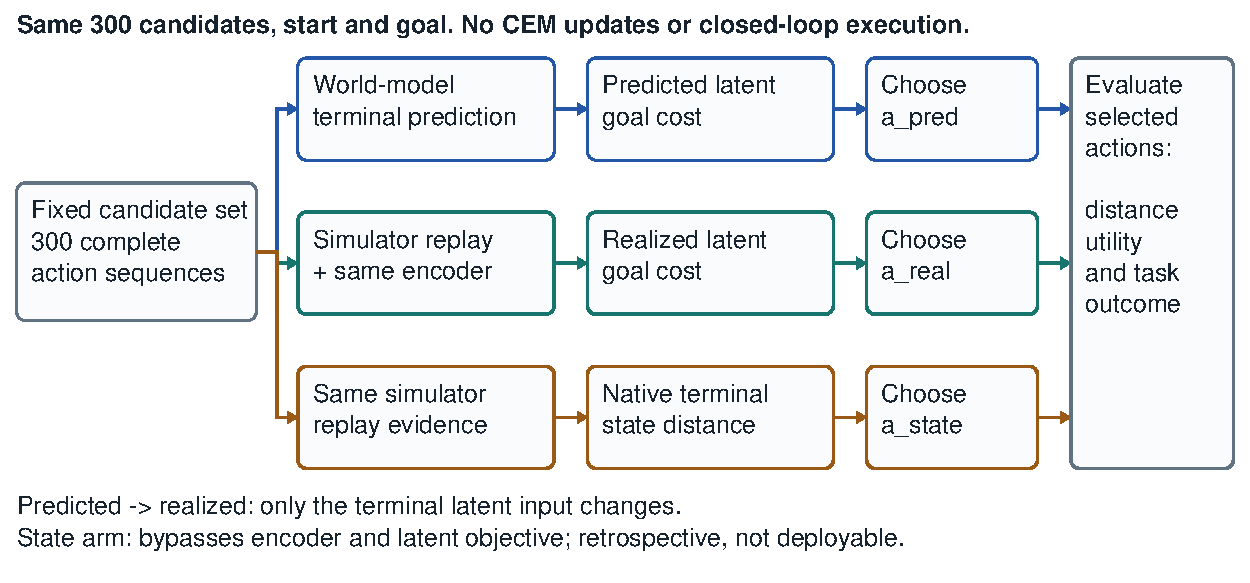
\includegraphics[width=\linewidth]{audit_overview.pdf}
\caption{The same fixed candidates, initial state and goal feed all selectors.
Endpoint substitution changes only the input to the fixed latent cost.
The separate hindsight state selector bypasses the learned representation and
objective together (Section~\ref{sec:state}); it is not a deployable policy.
A changed choice is not automatically a physical failure.}
\label{fig:audit}
\end{figure}

\subsection{Near ties measure decision ambiguity, not model uncertainty}

Collapse exact duplicate physical action sequences, retaining the minimum
predicted cost per distinct sequence. Let $c_{(1)}$ and $c_{(2)}$ be the
lowest two remaining predicted costs. Define the ambiguity score $A$ by
\begin{equation}
 \begin{aligned}
 m&=\frac{c_{(2)}-c_{(1)}}{\max\{\operatorname{IQR}(C_{\mathrm{pred}}),\epsilon\}},\\
 A&=-\log_{10}\!\left(\max\{m,\epsilon\}\right),\qquad \epsilon=10^{-12}.
 \end{aligned}
 \label{eq:near}
\end{equation}
Larger $A$ means a closer predicted race relative to within-set score spread.
The score uses predicted costs and action identity only; it does not use
realized costs, current-record prediction errors, or physical outcomes.
IQR normalization is not an estimate of model-error variance.

The motivation is algebraic. Write
$\delta_i=C_{\mathrm{pred}}(i)-C_{\mathrm{real}}(i)$.
If $i_{\mathrm{pred}}$ beats candidate $b$ by predicted margin
$g=C_{\mathrm{pred}}(b)-C_{\mathrm{pred}}(i_{\mathrm{pred}})>0$,
their order reverses after substitution exactly when
$\delta_b-\delta_{i_{\mathrm{pred}}}>g$.
A margin supplies neither a perturbation distribution nor the physical
value of either action. Within either latent block, dimension $d$ and
error $e_i=\hat z_i-z_i$ give the exact cost difference
$2(z_i-z_g)^\top e_i/d+\|e_i\|_2^2/d$.
The two blocks combine with the weights in Eq.~\ref{eq:cost}. This explains
score movement algebraically, not physical behavior causally.

\subsection{Separate validation targets}

\paragraph{Selector instability.}
The primary diagnostic target is the event
$a_{\mathrm{pred}}\ne a_{\mathrm{real}}$. In Push-T, every fitted
threshold or probability model excludes the evaluated trajectory, including
both models, all offsets, and all seeds. Each leave-one-trajectory-out (LOTO)
fold sets a model-specific 75th-percentile $A$ threshold on its 19 training
trajectories. A fixed-ridge logistic model (penalty $10^{-4}$, unpenalized
intercept) uses model identity and training-fold-standardized $A$. Baselines
use training-fold prevalence, model-specific prevalence, and model identity
plus negative log raw margin. The raw-score AUROC and the fitted probability
model's AUROC are reported separately.

\paragraph{Physical consequence.}
For candidate sets with varying physical outcomes, we evaluate the predicted selector's
normalized regret
\begin{equation}
 \mathcal{R}_{\mathrm{pred}}^Y=
 \frac{\max_iY(a_i)-Y(a_{\mathrm{pred}})}
      {\max_iY(a_i)-\min_iY(a_i)}.
 \label{eq:regret}
\end{equation}
Regret normalization is undefined when all candidate outcomes are equal.
Flagged-minus-unflagged
regret tests whether the screen identifies poorer original decisions. This
differs from asking whether replacing the predicted choice with the
realized-endpoint choice would worsen an outcome. That is a hypothetical
intervention, not risk of the deployed predicted selector. Selective evaluation retains scores below the model-specific
25th, 50th, and 75th percentiles learned on the other trajectories, plus all
records at full coverage. We report achieved coverage, selector-switch rate,
and physical regret separately.

The near-tie analysis is post-hoc. Its definitive protocol followed an initial
smoke test and a methodological amendment, rather than a preregistration before
the original study. Bootstrap intervals use 10,000 whole-trajectory resamples;
they condition on the chosen score and saved out-of-fold predictions and do
not refit the cross-validation pipeline or account for post-hoc score choice.

\section{Study design and evidence accounting}

We use released JEPA-WM and DINO-WM checkpoints~\citep{terver2026drives,pmlr-v267-zhou25t}.
Both use DINOv2 visual features; two predictors are not two independent
representation families. Every record contains 300 initially sampled action sequences,
each consisting of six model actions expanded to 30 physical steps. All
comparisons are within frozen candidate sets, not optimized CEM populations or
closed-loop rollouts.

\paragraph{Push-T.}
A planar agent pushes a T-shaped block toward a target pose. The issued
schedule crosses 20 validation trajectories, five outcome-blind offsets,
three proposal seeds, and two predictors (600 model records). We use negative
official terminal-state distance $U_{\mathrm{dist}}$ and cumulative coverage reward $R_{\mathrm{task}}$.
$U_{\mathrm{dist}}$ is negative Euclidean distance over seven coordinates: agent position, block
position, raw block angle, and agent velocity. It is not block-pose error
alone. Its goal is generated by replaying the 30-step dataset segment.
$R_{\mathrm{task}}$ instead sums 30 official rewards, each
$\min\{\mathrm{coverage}/0.95,1\}$, for overlap with the environment's fixed
target pose $(256,256,\pi/4)$. That target is not reassigned to the replay
endpoint. Thus the distance goal and coverage target have different
definitions; improving one outcome need not improve the other.

The physical-comparison mask contains 562 valid model records in 281 paired
cells. Overall, 577 records pass the artifact, complete-rollout, finite-score
and selector checks; validity does not mean task success. For the original physical contrasts, each cell
averages both models, each trajectory uses its fixed 15-cell denominator,
and invalid or unmatched cells contribute zero contrast evidence, not physical
outcomes of zero. For example, 14 matched cells each contributing $+1$ give a
trajectory contrast of $14/15$, not an observed-cell mean of $1$. This changes
the estimand and does not remove missingness bias. Inference uses 10,000 trajectory-bootstrap draws and exact
trajectory sign flips, assuming sign symmetry. Holm correction is separate
for the two realized-minus-predicted outcomes and the two
predicted-minus-uniform outcomes. Nineteen of
20 trajectories have at least 12 matched cells; the remaining trajectory stays
under the frozen evidence rule. The exploratory diagnostic instead reports
valid-row rates and AUROCs with trajectory-clustered intervals.

An outcome-blind infrastructure amendment retried 169 CUDA-cascade failures
before scientific-array inspection, retaining 23 invalid scheduled records.
Because this departed from the locked no-retry rule, the study is explicitly
recovery-augmented. Original attempts, recovery receipts, and an
original-completions-only sensitivity remain retained. The original-only subset
has 408 matched records and fails the original support requirement. Appendix~\ref{app:protocol}
states that rule, recovery eligibility, and the remaining missingness caveat.

\paragraph{Wall transfer.}
In a separate simulated navigation environment, 30 case seeds, three candidate set
seeds, and two task-specific predictors yield 180 issued rows. There are
179 verified valid rows and one retained scientific-validation failure. Its
compact failure ledger does not establish the specific failed criterion. Primary
physical effects use 174 rows from 29 complete six-row cases, exceeding the
prespecified minimum of 27; failed outcomes are not imputed. Each case
averages its candidate sets and predictors before 10,000 whole-case bootstrap draws
and 100,000 paired sign flips with a $+1$ correction. Native utility is
negative terminal distance; binary success uses the released distance
threshold of 4.5. Two-outcome Holm families are defined as in Push-T.

The Wall plan and near-tie rule were frozen before Wall outcomes. We apply
the Push-T-derived thresholds $A\ge1.289908$ for JEPA-WM and
$A\ge1.461432$ for DINO-WM without retuning. Switch AUROCs use all 179 valid
rows; the physical flagged comparison uses complete cases. Wall uses stable
first-minimum selection. Push-T's strict-selection validity rules can abstain
on ambiguous minima, so this transfer is not a pooled identical-protocol
estimate. Both environments use common candidates across the two selectors.

\section{Results}

\subsection{Near ties discriminate switching, not higher original regret}

On 562 matched Push-T rows, 331 actions switch. The raw near-tie score has
AUROC $.714$ (95\% CI $[.665,.762]$); the fitted LOTO probability model has
AUROC $.706$. The held-out quartile rule flags 142/562 rows (25.3\%): switch
rates are 82.4\% versus 51.0\%, a ratio of 1.62 ($[1.44,1.82]$).

\begin{table}[t]
\centering\small
\caption{Push-T out-of-fold switch-probability models on 562 matched rows.
Lower Brier score and log loss are better. Normalization adds little beyond
the raw-margin comparator; all models target switching, not physical risk.}
\label{tab:probability}
\begin{tabular}{lrrr}
\toprule
Predictor & AUROC & Brier score & Log loss \\
\midrule
Training-fold prevalence & $.410$ & $.243$ & $.679$ \\
Model-specific prevalence & $.451$ & $.243$ & $.680$ \\
Model identity + raw log margin & $.701$ & $.215$ & $.624$ \\
Model identity + near-tie score $A$ & $.706$ & $.214$ & $.622$ \\
\bottomrule
\end{tabular}
\end{table}

Adding $A$ to model identity improves Brier score from $.243$ to $.214$;
the paired trajectory-average loss-difference interval is $[-.043,-.016]$.
However, improvement over raw log margin is not established (Brier-difference
CI $[-.0054,.0037]$). Prevalence baselines vary across held-out folds, so their
pooled AUROC need not be $.5$ even without within-fold discrimination.

Raw-score AUROCs are $.734$ for JEPA-WM and $.691$ for DINO-WM. Recomputing
winners with maximum absolute normalized action coordinate at most $3$ gives $.696$;
the 408 model-matched original-completion rows give $.709$.

\begin{figure}[t]
\centering
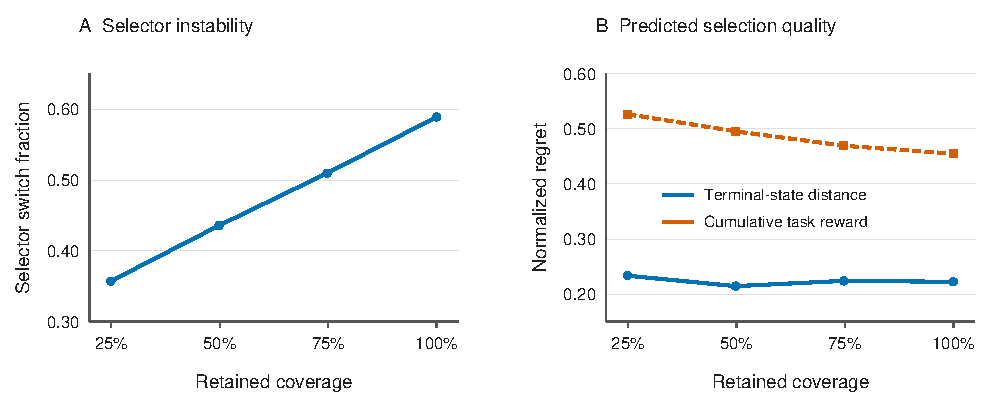
\includegraphics[width=\linewidth]{selective_diagnostic.pdf}
\caption{Push-T selective evaluation from the frozen post-hoc analysis.
Thresholds are set on other trajectories; the horizontal axis uses achieved
coverage. Retaining less ambiguous candidate sets lowers selector-switch rate (left),
but the original selector's physical regret does not improve consistently
(right). Curves are descriptive valid-row means, not confidence bands or
measured benefits from a deployed fallback. Lower vertical-axis values are better.}
\label{fig:selective}
\end{figure}

The physical check does not support labeling the flag as physical risk.
Flagged-minus-unflagged normalized regret for predicted selection is $-.007$
for distance utility (95\% CI $[-.039,.026]$) and $-.056$ for task reward
($[-.143,.026]$).
At roughly 25\% retained coverage, switch rate drops from $.589$ to $.357$,
but mean normalized distance regret is $.233$ versus $.222$ at full coverage,
and mean normalized reward regret is $.526$ versus $.455$
(Fig.~\ref{fig:selective}). Thus a cleaner
switch-rate curve is not evidence of a better physical decision policy.
This does not establish independence between regret and ambiguity.

\subsection{Prospective transfer preserves the limited target}

Wall selectors switch in 100/179 valid rows (55.9\%). The Push-T-frozen score
has descriptive pooled AUROC $.727$, compared with $.735$ for negative raw
margin. The transferred normalized score therefore does not outperform the
simple baseline. These point estimates do not establish probability calibration
under environment shift.

On complete Wall cases, the frozen thresholds flag 35/174 rows; 19 cases
contain both flagged and unflagged rows. The paired flagged-minus-unflagged
effect in the predicted-selected signed native gap is $+.393$
(95\% case-bootstrap CI $[-1.704,2.627]$). This gap is
$\min_i D(s_i,s_g)-D(s_{i_{\mathrm{pred}}},s_g)\le0$, so more negative means worse selection. Its sign
convention differs from positive regret in Eq.~\ref{eq:regret}. The comparison
does not establish greater physical shortfall in flagged rows.

\subsection{Endpoint substitution is not established physical recovery}

\begin{table}[t]
\centering\small
\caption{Original physical comparisons. Each cell reports an effect,
unadjusted 95\% cluster-bootstrap interval, and within-family Holm-adjusted
sign-flip value $p_H$. Positive favors the first named selector. Push-T uses
20 trajectories with the fixed denominator; Wall uses 29 complete cases.}
\label{tab:effects}
\begin{tabular}{@{}p{.18\linewidth}p{.37\linewidth}p{.37\linewidth}@{}}
\toprule
Outcome & Realized minus predicted & Predicted minus uniform\\
\midrule
\raggedright Push-T distance utility & $-5.30$ [$-9.64,-.71$];\newline $p_H=.0755$
 & $+48.70$ [$40.47,56.43$];\newline $p_H=7.63\!\times\!10^{-6}$\\
\raggedright Push-T cumulative reward & $+.042$ [$-.176,.240$];\newline $p_H=.701$
 & $+.761$ [$.420,1.117$];\newline $p_H=4.02\!\times\!10^{-4}$\\
\raggedright Wall distance utility & $-.254$ [$-.909,.364$];\newline $p_H=.923$
 & $+12.363$ [$10.900,13.755$];\newline $p_H=2.00\!\times\!10^{-5}$\\
\raggedright Wall completion & $+.0287$ [$0,.0805$];\newline $p_H=.923$
 & $+.0170$ [$0,.0454$];\newline $p_H=.501$\\
\bottomrule
\end{tabular}
\end{table}

Predicted scoring beats uniform on both Push-T outcomes and Wall native
utility, but endpoint substitution does not pass the respective two-outcome
tests (Table~\ref{tab:effects}). In Push-T, the adverse distance-utility estimate is
descriptive evidence worth explaining, not a demonstrated null effect. Its
marginal bootstrap interval excludes zero whereas the separate Holm-adjusted
sign-flip test does not pass $.05$; these are not an inverted CI/test pair.
The reward-effect interval permits effects in either direction, so neither equivalence
nor guaranteed harm follows. The negative distance-utility pattern is descriptively larger
for JEPA-WM, without a preregistered model-interaction claim.

In Wall, only two of 29 complete cases contain any successful candidate.
Predicted selection succeeds in 3/174 records and realized-endpoint selection
in 8/174. Repeated rows are not
independent success trials. This sparsity limits the success endpoint and
does not establish success equivalence.

Across all 577 valid Push-T records, 337 selectors switch. Only 48
and 38 switches reverse the strict predicted-versus-distance-best and
predicted-versus-reward-best pairwise ordering in the recovery-aligned direction.
These are specific best-candidate pair diagnostics, not counts of all
physically beneficial switches. They use the broader diagnostic population,
not the 562-row mask used for the main near-tie evaluation.

\subsection{Physical-component and score-scale checks}

\begin{table}[t]
\centering\small
\caption{Post-hoc component effects: realized minus predicted selection.
All component utilities are higher-is-better. The
five-outcome family was specified before inspecting component outcomes.
Intervals are unadjusted; $p_H$ corrects across all five components. These
are separate utilities, not additive contributions to mean unsquared distance.}
\label{tab:components}
\begin{tabular}{lrr}
\toprule
Component utility & Effect [95\% CI] & $p_H$ \\
\midrule
Agent position & $-1.817$ [$-4.564,.971$] & $.232$ \\
Block position & $+1.267$ [$.480,2.176$] & $.0203$ \\
Circular block angle & $+.0325$ [$.0197,.0471$] & $.000210$ \\
Agent velocity & $-5.809$ [$-10.523,-1.187$] & $.0957$ \\
Terminal coverage & $+.00901$ [$.00035,.01696$] & $.110$ \\
\bottomrule
\end{tabular}
\end{table}

Push-T's whole-state distance combines unlike coordinates. To avoid reading an
adverse distance-utility effect as uniformly worse manipulation, a separate post-hoc analysis uses
negative Euclidean position/velocity errors, negative circular angle error,
and final-step coverage. Under the same fixed trajectory aggregation,
block-position and circular-orientation errors improve, while agent-state
point estimates worsen (Table~\ref{tab:components}). Circular angle is not
the raw-angle coordinate used by native distance. Agent-state and terminal-coverage effects
do not pass the five-component Holm threshold.

On the descriptive squared-distance scale, the mean component errors at the
predicted-selected endpoint minus those at the realized-selected endpoint
are $-477.2$ for agent position, $+79.2$ for block position,
$+.226$ for raw angle, and $-1497.0$ for agent velocity. Their row-wise sum
is exact (maximum residual $3.64\times10^{-11}$). These native-coordinate
contributions are not unit-invariant and do not add to the mean unsquared
distance-utility effect. They locate the measured trade-off; they do not causally identify
an encoder, predictor, or objective defect.

Prediction error is material relative to candidate set spread. Across the 562 matched
rows, the trajectory-weighted mean within-candidate set $\rho(C_{\mathrm{pred}},C_{\mathrm{real}})$ is $.858$
(95\% CI $[.839,.875]$). The mean per-candidate set median $|C_{\mathrm{pred}}-C_{\mathrm{real}}|$ is $.0505$;
mean per-candidate set ratios to predicted- and realized-score IQR are $.339$ and
$.316$. Broad rank agreement can therefore coexist with frequent top-choice
changes. These offline scale summaries are not inputs to $A$ and are not
uncertainty estimates.

\subsection{A separate hindsight state-distance diagnostic}
\label{sec:state}

To examine what remains after terminal prediction correction, a later post-hoc
analysis chooses $i_{\mathrm{state}}=\arg\min_i D(s_i,s_g)$, where $D$ is the
stored native terminal-state distance. It evaluates both physical outcomes
at that same selected sequence. This selector uses realized simulator outcomes,
jointly bypasses the learned encoding and latent objective, and is not
deployable. It neither estimates model uncertainty nor identifies which
component causes the remaining regret.

Using the original paired-cell and complete-case masks, it improves distance
utility relative to realized-latent selection by $69.814$ in Push-T
(unadjusted 95\% trajectory-bootstrap CI $[62.326,77.641]$) and $5.643$ in
Wall ($[3.861,7.664]$). Improvement in its selected distance is guaranteed by
construction; the magnitudes describe fixed-set headroom. Push-T cumulative
reward instead declines by $0.838$ ($[-1.222,-0.460]$). The different target
definitions and temporal objectives prevent assigning that trade-off to an
encoder defect or a single causal mechanism.

On Wall it adds no observed completions beyond realized-latent selection:
both select success in 8/174 repeated model records, versus 3/174 for predicted
selection. Completion thresholds the same distance minimized by the hindsight
selector, and only two complete cases contain a successful candidate. Equal
observed completion therefore reflects captured candidate support, not
population equivalence. The new analysis uses 10,000 whole-cluster resamples
and no new $p$-values; it does not replace the original inference in
Table~\ref{tab:effects}. Appendices~\ref{app:original} and~\ref{app:models}
separately report original inference and all model-specific new contrasts.

\section{Implications, limitations, and reproducibility}

A possible use, not a validated policy, is a \emph{candidate verification trigger}: identify where
additional evaluation might change a latent selector's answer. The audit does
not establish which verifier or fallback to use, how much it should cost, or
whether it would improve outcomes. A prospective intervention must measure
physical benefit at a fixed verification budget, not just fewer selector
disagreements. Likewise, a small margin is not evidence of epistemic or
aleatoric uncertainty: even a perfectly known deterministic objective can
contain near ties.

Scope remains limited to short open-loop initial candidate sets in one manipulation
and one navigation environment, related DINOv2-based predictors, and simulator
outcomes. There is no independent representation-family study, optimized-CEM
evaluation, hardware validation, or safety guarantee. Raw margin remains a
competitive comparator. Push-T recovery augmentation, finite cluster counts,
post-hoc diagnostic selection, conditional bootstrap intervals, and sparse
Wall success constrain the conclusions.
The new retrospective state-selector analysis is also post-hoc and does not
supply independent validation of the near-tie screen or identify a faulty
encoder or objective.

The retained evidence includes candidate scores, physical outcomes, action
identities, selector indices, protocol versions, and failure records. A compact
Wall CPU recomputation artifact contains 53,700 model--candidate records and
recomputes saved selectors, complete-case effects, and fixed-score AUROCs
without GPU inference. This is analysis reproducibility, not reproduction of
training or a full planning pipeline. The new diagnostic package remains
locally retained for release; we do not claim that it has already been
publicly uploaded. Appendix~\ref{app:config} records preprocessing, action
normalization, dataset/goal construction, and source/checkpoint bindings;
Appendix~\ref{app:repro} states the recomputation scope and remaining gaps.
AI tools assisted implementation and
drafting; the authors are responsible for verification and all claims.

\section{Conclusion}

Near-tie scores can identify action choices that are sensitive to realized
endpoint substitution without identifying higher physical regret. Push-T
held-out evaluation and a frozen Wall transfer support the former association,
not a physical-risk claim or superiority over raw margin. Decision-aware
uncertainty evaluation should specify the event being predicted and separately
test its physical consequences.

\clearpage
\bibliography{references}
\clearpage
\appendix
\section{Notation and interpretation glossary}
\label{app:glossary}

\begin{table}[h]
\centering
\begin{tabular}{@{}p{0.27\linewidth}p{0.69\linewidth}@{}}
\toprule
Symbol or term & Meaning\\
\midrule
$a_i$ & Candidate $i$: a complete 30-step physical action sequence.\\
Endpoint $s_i$ & State after executing all actions in candidate $i$.\\
$z_i$, $\hat z_i$, $z_g$ & Encoded realized endpoint, predicted terminal latent, encoded goal.\\
$C_{\mathrm{pred}}$, $C_{\mathrm{real}}$ & The same latent goal cost evaluated on predicted or encoded realized endpoints.\\
$a_{\mathrm{pred}}$ & Candidate selected by predicted latent cost.\\
$a_{\mathrm{real}}$ & Candidate selected by realized-endpoint latent cost; retrospective, not a physical optimum.\\
$a_{\mathrm{state}}$ & Candidate minimizing realized native terminal distance; retrospective and non-deployable.\\
$D$, $U_{\mathrm{dist}}$ & Native distance and its negative, the higher-is-better distance utility.\\
$R_{\mathrm{task}}$ & Cumulative official Push-T coverage reward or Wall binary completion.\\
Record & One model, initial-state/goal instance, and proposal seed, with 300 candidates.\\
Paired cell & One Push-T trajectory offset and seed with valid records for both models.\\
Cluster & A scheduled Push-T trajectory or a complete Wall case; the resampling unit.\\
Initial candidates & Samples before any CEM distribution update; historically called an ``iteration-0 menu'' in code.\\
\bottomrule
\end{tabular}
\end{table}

\section{Original inference, unchanged}
\label{app:original}

Table~\ref{tab:original} retains the original pooled point estimates, percentile
intervals, and Holm-adjusted sign-flip values. Push-T uses all 20 scheduled
trajectory contrasts, 10,000 trajectory-bootstrap draws, and enumeration of
all $2^{20}$ sign assignments for its two-sided paired test. Wall uses 29
complete-case contrasts, 10,000 case-bootstrap draws (seed 20260911), and
100,000 random sign assignments with the $+1$ correction (seed 20260912).
Holm adjustment covers two outcomes separately for endpoint correction and
predicted-minus-uniform selection within each environment. Push-T's bounded
candidate sensitivity has its own originally declared two-outcome family.
The exact test requires sign symmetry of cluster contrasts under the null.
No new state-selector comparison has been added to those original families.

\begin{table}[h]
\caption{Unchanged original inference. Intervals are marginal 95\% cluster
bootstrap intervals; $p_H$ is the original within-family Holm-adjusted value.}
\label{tab:original}
\centering\small
\begingroup
\setlength{\tabcolsep}{3pt}
\begin{tabular}{lllrr}
\toprule
Environment & Contrast & Outcome & Effect [95\% CI] & $p_H$\\
\midrule
Push-T & Realized $-$ predicted & Distance utility & $-5.299\ [-9.635,-0.706]$ & .075539\\
 & & Reward & $+0.04183\ [-0.17569,0.24024]$ & .701128\\
 & Predicted $-$ uniform & Distance utility & $+48.702\ [40.473,56.434]$ & $7.6294\!\times\!10^{-6}$\\
 & & Reward & $+0.76099\ [0.42033,1.11714]$ & .00040245\\
Wall & Realized $-$ predicted & Distance utility & $-0.25365\ [-0.90933,0.36436]$ & .923091\\
 & & Completion & $+0.02874\ [0,0.08046]$ & .923091\\
 & Predicted $-$ uniform & Distance utility & $+12.36271\ [10.90015,13.75461]$ & $1.99998\!\times\!10^{-5}$\\
 & & Completion & $+0.01705\ [0,0.04544]$ & .501395\\
\bottomrule
\end{tabular}
\endgroup
\end{table}

The new diagnostic uses seeds 20261002 (Push-T) and 20261003 (Wall), with
10,000 whole-cluster draws shared by its three contrasts and both outcomes
within each environment. These intervals quantify the new post-hoc comparisons
and do not replace the original test decisions. Recomputing the original
results is a required preflight check before generating the new results.

\section{Model-specific descriptive comparisons}
\label{app:models}

Table~\ref{tab:models} uses the same retained cells, cluster definitions,
denominators, and common bootstrap draws as the pooled post-hoc analysis.
Each model estimate compares a latent selector with the same physical state
selector on matched sets. Repeated state-selected outcomes do not provide a
second physical experiment. All entries are descriptive; differences between
their confidence intervals are not model-interaction tests.

\begin{table}[h]
\caption{Post-hoc model-specific effects with 95\% cluster-bootstrap
intervals. ``Real'', ``pred'', and ``state'' refer to the three defined selectors.}
\label{tab:models}
\centering\small
\begin{tabular}{lllrr}
\toprule
Task & Model & Contrast & $\Delta U_{\mathrm{dist}}$ [95\% CI] & $\Delta R_{\mathrm{task}}$ [95\% CI]\\
\midrule
Push-T & JEPA-WM & Real $-$ pred & $-9.330\ [-14.394,-4.557]$ & $+.081\ [-.130,.280]$\\
 & & State $-$ real & $+67.623\ [59.887,76.057]$ & $-.861\ [-1.271,-.453]$\\
 & & State $-$ pred & $+58.293\ [50.879,65.943]$ & $-.780\ [-1.169,-.407]$\\
 & DINO-WM & Real $-$ pred & $-1.268\ [-7.898,6.272]$ & $+.003\ [-.241,.237]$\\
 & & State $-$ real & $+72.005\ [63.922,80.083]$ & $-.815\ [-1.179,-.462]$\\
 & & State $-$ pred & $+70.737\ [64.052,77.512]$ & $-.812\ [-1.229,-.420]$\\
\addlinespace
Wall & JEPA-WM & Real $-$ pred & $-.655\ [-1.649,.215]$ & $+.0345\ [0,.0920]$\\
 & & State $-$ real & $+4.910\ [3.327,6.785]$ & $0\ [0,0]$\\
 & & State $-$ pred & $+4.255\ [3.001,5.839]$ & $+.0345\ [0,.0920]$\\
 & DINO-WM & Real $-$ pred & $+.148\ [-.724,.923]$ & $+.0230\ [0,.0690]$\\
 & & State $-$ real & $+6.376\ [4.222,8.825]$ & $0\ [0,0]$\\
 & & State $-$ pred & $+6.524\ [4.551,8.761]$ & $+.0230\ [0,.0690]$\\
\bottomrule
\end{tabular}
\end{table}

\section{Sampling, missingness, and the recovery amendment}
\label{app:protocol}

\paragraph{Push-T selection and support.}
The manifest selects validation trajectory indices 0--20 except 7, for 20
trajectories, without consulting audit outcomes. For a trajectory of length
$L$, its five offsets are $\lfloor k(L-31)/4\rfloor$, $k=0,\ldots,4$.
Only recorded sequence lengths select the offsets. Expert block-state motion
labels a secondary phase proxy but does not select or exclude records.
Each offset is paired with proposal seeds 1, 2, and 3 and both models.
The resulting 100 distinct initial-state/goal segments produce 300 offset--seed
cells and 600 scheduled model records. The manifest's historical
\texttt{segment\_count=300} includes proposal seeds.

For an outcome $Y$ (either $U_{\mathrm{dist}}$ or $R_{\mathrm{task}}$), let
$\delta_{tcm}$ be a specified selector contrast for trajectory $t$, cell $c$,
and model $m$. The cell indicator $I_{tc}$ equals one only when both model
records are valid under the original rules. The pooled trajectory contrast is
\begin{equation}
 \bar\delta_t=\frac{1}{2}\sum_{m=1}^{2}
          \frac{1}{15}\sum_{c=1}^{15} I_{tc}\delta_{tcm},
 \qquad \widehat\Delta=\frac{1}{20}\sum_{t=1}^{20}\bar\delta_t.
 \label{eq:cluster}
\end{equation}
Missing-cell terms are defined as zero \emph{contrast contributions}; the
formula does not assign a physical outcome to a missing action. The two-model
mask and fixed 15-cell denominator are preserved for every new contrast and
model split. Observed-cell means would answer a different question.
The original support requirement is at least 540 matched model records and
at least 18 trajectories with 12 or more matched cells. The retained study
has 562 matched records and 19 such trajectories, so it meets that requirement;
all 20 scheduled trajectories still enter Eq.~\ref{eq:cluster}.
Support gates require coverage of the scheduled experiment, not a positive
physical effect or a guarantee of adequate power. The original broad-recovery
rule additionally required passed integrity and repeat-stability checks;
positive pooled means and lower 95\% bounds, with Holm-adjusted $p<.05$, for
both outcomes under raw and bounded candidates; positive model-specific lower
bounds for both outcomes in both candidate sets; and no conflicting pooled
signs. Failure of any condition blocked the broad claim. Sampling, outcomes,
aggregation, tests, and this rule were recorded in the original locked protocol;
recovery was a later amendment, and the auxiliary and new state-selector
analyses are separately labeled post-hoc.

\paragraph{Infrastructure recovery.}
The Push-T protocol was recorded as locked on August 30, 2026 and prohibited
retries. Its original 600-record attempt ledger ended with 420 completed and
180 failed records. A fatal CUDA error had contaminated the persistent worker,
causing later untouched records to receive the same infrastructure error.
The recovery amendment mechanically selected 169 failed records with that
exact error message for at most one attempt each, in isolated processes.
The remaining failure classes were not eligible. The amendment states that
eligibility was fixed before inspecting scientific outcomes, preserving
candidate specifications and analysis rules, but this remains a deviation
from the original no-retry rule. Original failures remain in the ledger;
recovery neither deletes them nor makes them original completions.
The no-retry rule restricted opportunities to change retained evidence through
selective repeated attempts; the amendment does not retroactively satisfy it.
The recovery-augmented analysis has
577 valid and 23 invalid records, with 15 valid records unmatched across models.
Removing every recovery-sourced artifact leaves 408 matched records and only
14 trajectories meeting the original eligibility threshold: the original-only
subset fails the original support requirement. Its distance and reward effects
are $-5.39$ ($[-9.32,-1.40]$) and $-0.019$ ($[-0.212,0.160]$), respectively.
These are exploratory sensitivity estimates, not a restored confirmatory
analysis or evidence that missingness is ignorable. The 15 observed trajectory
groups used by a separate diagnostic are not 15 eligible primary clusters.

Earlier protocol versions are not scientific inputs to this analysis: v1.2
failed its prescribed RGB/serialization integrity check, and v1.3 failed
before usable measurements because a replay-encoding helper lacked its
required model argument. The v1.4 source and evidence are separately bound;
no earlier-version result is reused. The retained protocol, amendment, and
ledgers make this history inspectable but do not constitute an independently
registered timestamp for the declared outcome-blind sequence.

\paragraph{Wall selection and missingness.}
Case seeds 2026091100--2026091129 generate the 30 initial-state/goal cases.
Engineering seeds 2026091001 and 2026091002 are excluded from the study.
The wall location is 32 and door location 30 in the underlying 65-pixel
environment. Each case contains seeds 1--3 and both models. One JEPA-WM
record, case \texttt{wall\_028}, seed 1, failed scientific validation and was
not retried. Its entire case is excluded from the complete-case physical
analysis. The remaining five valid records contribute only to all-valid
descriptions. Case contrasts average the six model--seed records equally;
the 29 case means are the inferential units. This restriction does not rule
out difficulty-dependent missingness.
The retained failure ledger labels this failure \texttt{scientific\_or\_child}
but supplies no error message, so its specific failed criterion is not
established by that ledger.

\paragraph{Integrity and ties.}
Original Push-T validity required finite production arrays, decomposition
residuals at most $10^{-8}$, and score reproduction within $2\times10^{-5}$
with zero relative tolerance. Re-encoding serialized observations at chunk
sizes eight and four had to preserve scores within that tolerance and the
latent minimum tie sets exactly. Original repeat and provenance checks also
applied. Execution completion alone therefore did not imply scientific
validity; a valid record still needed its partner for paired analysis.
The new preflight checks cover all 780 unique scheduled records: 756 valid
and 24 invalid across both environments. They verify candidate counts,
selectors, stored physical arrays, cross-model agreement, and the original
headline analysis before new computation. Push-T's original latent selectors
require a unique minimum under absolute tolerance $10^{-10}$ and relative
tolerance $10^{-8}$; otherwise that record is invalid. Wall's latent selectors
use the first exact minimum. The new state selector also uses the first exact
minimum. No exact minimum ties or duplicate physical sequences occur in the
retained valid candidate sets; synthetic tests cover deterministic tie
handling. Cross-model identity is established by arrays, not assumed from
shared random-seed labels.

\section{Model and environment configuration}
\label{app:config}

\paragraph{Visual encoding.}
Both models in both tasks load \texttt{dinov2\_vits14} from
\texttt{dinov2\_vits14\_pretrain.pth}: a ViT-S/14 with 384-dimensional patch
features. Raw RGB is divided by 255 and resized to $224\times224$ using
bilinear interpolation with \texttt{align\_corners=False}. The audit loaders
fix spatial scale and aspect-ratio augmentation ranges to $(1,1)$ and disable
flips, motion augmentation, automatic augmentation, and random erasing.
DINO-WM then uses per-channel mean and standard deviation $(0.5,0.5,0.5)$.
JEPA-WM uses mean $(0.485,0.456,0.406)$ and standard deviation
$(0.229,0.224,0.225)$. Sharing backbone weights therefore does not mean that
the models receive identically normalized inputs. Each model's preprocessing
is fixed between its predicted and realized costs.

\paragraph{Proprioception and actions.}
Push-T proprioception contains the agent's two-dimensional position and
velocity (four coordinates), not block pose. Wall proprioception is the
two-dimensional agent position. After the released coordinate normalization,
the frozen proprioceptive encoder is a kernel-one, stride-one convolution,
equivalent to a per-time-step affine map. Its output dimension is 20 for
DINO-WM on Push-T and 10 on Wall, versus 16 for JEPA-WM on both tasks.
Table~\ref{tab:normalization} gives the environment normalization constants;
the operational meaning of action normalization is
$a_{\mathrm{physical}}=\sigma_a\odot a_{\mathrm{normalized}}+\mu_a$.
Consequently, candidate zero is a normalized-mean sequence, not necessarily
a physical no-op. Gaussian proposals are unbounded in normalized coordinates;
the bounded sensitivity is defined separately, not silently substituted.

\begin{table}[h]
\caption{Released environment normalization constants, rounded here for
readability. Full-precision values remain in the bound dataset registry.}
\label{tab:normalization}
\centering\small
\begin{tabular}{@{}p{0.10\linewidth}p{0.32\linewidth}p{0.50\linewidth}@{}}
\toprule
Task & Quantity & Values\\
\midrule
Push-T & Action mean & $(-0.0087,\ 0.0068)$\\
 & Action standard deviation & $(0.2019,\ 0.2002)$\\
 & Proprioception mean & $(236.61549,\ 264.56741,\ -2.93032,\ 2.54308)$\\
 & Proprioception standard deviation & $(101.12020,\ 87.01120,\ 74.84556,\ 74.14009)$\\
Wall & Action mean & $(-0.00556462,\ 0.01319782)$\\
 & Action standard deviation & $(0.75233287,\ 0.74668980)$\\
 & Proprioception mean & $(31.89451,\ 31.81402)$\\
 & Proprioception standard deviation & $(17.66352,\ 17.27517)$\\
\bottomrule
\end{tabular}
\end{table}

The model horizon is six, action dimension ten, physical action dimension two,
and frame grouping five, giving 30 executed actions with
\texttt{action\_skip=1}. Initial image and proprioceptive history lengths are
one; rollout context is two. The objective is terminal visual MSE plus
$0.1$ proprioceptive MSE, with \texttt{sum\_all\_diffs=False}.
Push-T samples with a PyTorch generator on the initial latent's device;
Wall uses a CPU generator with shape $[6,300,10]$ before permutation.
Both use standard-normal proposals, but their random streams should not be
assumed identical across environments.

\paragraph{Dataset and goals.}
Push-T uses \path{data/pusht_noise/val} in the retained official source tree.
The simulator starts from \texttt{states[offset]} with the recorded shape,
and replays the 30 recorded relative actions using environment seed 1 to
generate the goal. The goal is not merely a frame extracted from the dataset
video. Wall cases are generated from the fixed random-state seeds described
above rather than validation-trajectory offsets. The capture routine
\texttt{run\_case} in \path{experiments/wall_decision_audit.py} calls the released
\texttt{WallEnvWrapper.sample\_random\_init\_goal\_states}, which delegates to
\texttt{DotWall.generate\_random\_state} in
\path{evals/simu_env_planning/envs/wall_env/envs/wall.py} under the bound
Wall configuration. It samples positions uniformly on opposite sides of the
wall within padded boundaries, reversing travel direction with probability
one half. These routines, not the seed alone, define case generation.

\paragraph{Source and checkpoint bindings.}
The official JEPA-WM source commit is
\nolinkurl{13cf1d9c7e476f53c17714d2e0f1dc239a883ce0};
the DINOv2 source commit is
\nolinkurl{b194f00db6136677fc8a4cc2ef2168f7699dfba2}.
The recorded Wall model-repository revision is
\nolinkurl{9b9c41ef249466630dbf1a20e78391865d07b3b9}.
The checkpoint filenames and SHA-256 digests are:
\begin{itemize}
\item \texttt{dino\_wm\_pusht.pth.tar}:\\
\texttt{8ec9cb05f22812d7f12e3c216b0637f4}\allowbreak\texttt{1641055c0653e503e2746edb981b550f}.
\item \texttt{jepa\_wm\_pusht.pth.tar}:\\
\texttt{9beca3eafe0739c3b3adb5d734fa435c}\allowbreak\texttt{cbda0fea8a65d53d4cccec176aaaa0eb}.
\item \texttt{dino\_wm\_wall.pth.tar}:\\
\texttt{ff170be5aec9249768be4a220d600b8f}\allowbreak\texttt{00a8589b2a78982ecf9273809f2767df}.
\item \texttt{jepa\_wm\_wall.pth.tar}:\\
\texttt{8efb0623cfba1cb3ca210de26f7579c8}\allowbreak\texttt{3dd24936635f11989c515afcb23bea1e}.
\end{itemize}
The DINOv2 weight-file digest is
\texttt{b938bf1bc15cd2ec0feacfe3a1bb553f}\allowbreak\texttt{e8ea9ca46a7e1d8d00217f29aef60cd9};
the recorded loaded state-dictionary digest is
\texttt{5bb315664719c85935c4b67a0f8faef9}\allowbreak\texttt{d01b7dfb57ffbecef1c062f7b4e4aa35}.
The Push-T dataset archive digest is
\texttt{442f5dee246edf670964ed7bdecd2486}\allowbreak\texttt{83cd6d00580fa0e4d458abb53f92da08}.

These facts are bound by
\path{experiments/official_pusht_v14_manifest.json}
(\texttt{selection}, \texttt{protocol}, \texttt{source\_bundle});
\path{output/source/physical_ai_supplement/official_pusht_v14_certificate_issuance.json}
(model, encoder, and data bindings);
\path{experiments/wall_audit_20260910/protocol.json};
\path{experiments/wall_audit_20260910/execution_bindings.json}; and
\path{output/wall_recompute_20260910_v3/metadata/provenance.json}.
The official planning configurations lie under
\path{configs/evals/simu_env_planning/}, with task directories \texttt{pt}
and \texttt{wall}, model directories \texttt{dino-wm} and \texttt{jepa-wm},
and names ending
\path{L2_cem_sourcedset_H6_nas6_ctxt2_r224_alpha0.1_ep96_decode.yaml}
for Push-T or the analogous \texttt{sourcerandstate} name for Wall.
Normalization constants are in
\path{app/plan_common/datasets/__init__.py} of the bound source tree.
Checkpoint training epochs, training seeds, and complete training-data
provenance are not established by these retained audit bindings; we do not
infer them from filenames.

\section{Earlier sensitivities and exact score accounting}
\label{app:sensitivity}

These analyses predate the state-selector extension and retain their original
status and numerical summaries. They are not new experiments for this revision.
The bounded-candidate and original-completions-only sensitivities concern
endpoint correction, not the new state-selector contrasts. We have not
reported an observed-cell-denominator analysis or an original-completions-only
state-selector analysis. Their absence leaves the corresponding robustness
questions unresolved; the existing sensitivities cannot establish that
missingness is ignorable for any contrast.

\paragraph{Bounded candidates.}
Restrict each set to sequences with maximum absolute normalized action
coordinate at most three. The original support requirement is at least 200
candidates and valid untied latent selectors. The realized-minus-predicted
effects are $-5.80$ in distance utility (95\% CI $[-11.00,-0.21]$,
Holm-adjusted $p=.111$) and $+0.115$ in reward ($[-0.093,0.314]$, $p=.296$).
The raw analysis remains primary; this sensitivity does not alter the new
state-selector definition or its candidate set.

\paragraph{Physical components.}
The component analysis was post-hoc, specified before inspecting component
outcomes. It uses the same 562 matched records, 281 cells, 20 trajectories,
and fixed denominators. Position and velocity utilities are negative
Euclidean distances to their goal components; angle utility is negative
circular absolute error, unlike the raw angle coordinate in native distance.
Terminal coverage reward is the last official reward, not the raw overlap
fraction reported separately by the environment. Holm adjustment covers these
five declared component tests.

\begin{table}[h]
\caption{Retained post-hoc Push-T component effects, realized minus predicted.
Intervals are original marginal 95\% trajectory-bootstrap intervals.}
\label{tab:appendix_components}
\centering
\begin{tabular}{lrrr}
\toprule
Component utility & Effect & 95\% CI & $p_H$\\
\midrule
Agent position & $-1.817$ & $[-4.564,.971]$ & .232\\
Block position & $+1.267$ & $[.480,2.176]$ & .0203\\
Circular block angle & $+.0325$ & $[.0197,.0471]$ & .000210\\
Agent velocity & $-5.809$ & $[-10.523,-1.187]$ & .0957\\
Terminal coverage & $+.00901$ & $[.00035,.01696]$ & .110\\
\bottomrule
\end{tabular}
\end{table}

For exact native squared-distance accounting, the mean predicted-selection
minus realized-selection contributions are $-477.2$ from agent position,
$+79.2$ from block position, $+0.226$ from raw angle, and $-1497.0$ from agent
velocity. Positive contributions mean realized selection reduces that squared
error. The maximum rowwise identity residual is $3.64\times10^{-11}$.
These mixed-unit squared contributions are not additive contributions to mean
unsquared distance utility, and they change under coordinate rescaling.

\paragraph{Stored-latent interpolation.}
For each candidate, the earlier post-hoc sensitivity scores
$(1-\lambda)\hat z_i+\lambda z_i$, for $\lambda=0,.1,\ldots,1$, with all
actions, goals, cost function, and physical outcomes otherwise unchanged. At
$\lambda=.5$, 38.4\% of matched-record choices change and the distance effect
is $-2.24$; at $\lambda=1$, these values are 58.9\% and $-5.30$.
All ten nonzero-$\lambda$ pooled distance point estimates are negative.
These aggregate points are not independent replicates, interpolated latents
need not represent realizable states, and no trainable correction is evaluated.

\paragraph{Score accounting is an identity, not a causal explanation.}
For either modality, write its prediction error as $e_i=\hat z_i-z_i$, with
dimension $d$. Then
\begin{equation}
 \frac{\|\hat z_i-z_g\|_2^2-\|z_i-z_g\|_2^2}{d}
 =\frac{2(z_i-z_g)^\top e_i}{d}+\frac{\|e_i\|_2^2}{d}.
 \label{eq:identity}
\end{equation}
Summing the two modalities with weights one and $0.1$ reconstructs
$C_{\mathrm{pred}}(i)-C_{\mathrm{real}}(i)$ exactly; subtracting two candidates'
identities reconstructs their margin change. The maximum residual in retained
Push-T records is $6.66\times10^{-16}$. Directional terms dominate magnitude
terms in 266 of 337 selector switches (78.9\%): the absolute directional
margin between the predicted and realized winners exceeds the absolute
magnitude margin after the visual and $0.1$ proprioceptive contributions are
combined. This is a record-level fraction, not cluster-level inference.
This explains algebraic score
movement, not its physical desirability or a causal failure mechanism.
The trajectory-weighted mean candidate-set Spearman correlation between the
two costs is $.858$ (95\% CI $[.839,.875]$); the mean per-set median absolute
cost difference is $.0505$, with mean ratio $.339$ to predicted-cost IQR.

\paragraph{Ranking summaries.}
Spearman correlates negative cost with higher-is-better outcome, using average
ranks for exact ties. Pairwise accuracy counts whether lower cost favors the
higher outcome, excluding pairs tied on either quantity. Per-record summaries
use the original paired-cell, equal-model, trajectory aggregation.
On bounded candidate support, the earlier descriptive distance-utility
Spearman correlations are .367 for predicted and .345 for realized scoring;
pairwise ranking accuracies are .599 and .591. Their normalized regrets are
.250 and .274. For cumulative reward, the corresponding pairs are .121/.124,
.469/.471, and .372/.359. For a higher-is-better outcome $Y$, normalized
regret of selection $a$ is
$(\max_iY(a_i)-Y(a))/(\max_iY(a_i)-\min_iY(a_i))$ when its denominator is
positive and the selector is defined. These summaries are descriptive and
do not establish ranking superiority.

\section{Secondary selector-instability diagnostic}
\label{app:neartie}

The earlier near-tie diagnostic targets whether $a_{\mathrm{pred}}$ and
$a_{\mathrm{real}}$ differ, not whether either fails physically. After
deduplicating physical actions and retaining the lowest predicted cost per
action, let $c_{(1)}$ and $c_{(2)}$ be the two lowest predicted costs.
The ambiguity score is
\begin{equation}
 -\log_{10}\!\left[\max\!\left\{
 \frac{c_{(2)}-c_{(1)}}{\max\{\operatorname{IQR}(C_{\mathrm{pred}}),10^{-12}\}},
 10^{-12}\right\}\right].
\end{equation}
The Push-T analysis was exploratory. Leave-one-trajectory-out logistic models
include model identity, with model-specific top-quartile thresholds learned
on the other 19 trajectories. Bootstrap intervals resample saved out-of-fold
predictions without refitting the complete pipeline, and do not account for
choosing this diagnostic after the primary result.

On 562 matched records, unfitted normalized-ambiguity-score AUROC is $.714$ ($[.665,.762]$), compared
with $.706$ for the fitted probability. The flagged group covers 25.3\% of
records and switches 82.4\% of the time versus 51.0\% outside it. However,
flagged-minus-unflagged normalized regret of $a_{\mathrm{pred}}$ is $-.007$ for distance utility
($[-.039,.026]$) and $-.056$ for reward ($[-.143,.026]$), neither establishing
greater physical regret.

Before the secondary Wall extension, model thresholds were frozen at
1.2899081787 for JEPA-WM and 1.4614315032 for DINO-WM, without Wall retuning.
Across all 179 valid records, the normalized score has AUROC $.727$ versus
$.735$ for raw margin. These descriptive estimates provide no normalization
advantage. The signed native gap is
$\min_iD(s_i,s_g)-D(s_{i_{\mathrm{pred}}},s_g)$; larger values mean less distance regret.
Its flagged-minus-unflagged effect is $+.393$
($[-1.704,2.627]$), using the 19 complete cases containing both groups.
Thus prospective freezing limits retuning but does not establish physical-risk
calibration, verification benefit, or an improvement over the simpler baseline.

\section{Artifacts, recomputation, and scope}
\label{app:repro}

The new analysis reads retained candidate scores, actions, terminal states
where available, native distances, and task outcomes. It verifies candidate
identity across models and reproduces the original effects, intervals, tests,
and families before computing the state-selector extension. Its numerical
review independently matched all 36 pooled/model-specific summaries and
intervals, valid-record selector outcomes, and cluster arrays. Original source
artifacts and result files are not overwritten.
These revision materials are retained locally for author release; this work
does not claim that the new package has already been publicly uploaded.

The camera-ready artifact directory
\path{output/task_native_selector_20261002/} contains the checked specification
and implementation reviews, \texttt{summary.csv}, \texttt{row\_effects.csv},
\texttt{cluster\_effects.csv}, \texttt{selection\_disagreements.csv},
\texttt{original\_results.json}, \texttt{physical\_support.json},
\texttt{RESULTS\_INTERPRETATION.md}, reproduction instructions, tests, and a
portable reproduction bundle. \texttt{SCIENTIFIC\_FREEZE.md} records the
pre-manuscript numerical freeze. The numerical summary SHA-256 is
\texttt{3eb5cb00fd7be3f9e01a6f1e6277b003}\allowbreak\texttt{02d0e1549c7d8c8845fba59570bb09c6}.
The reviewed result SHA-256 is
\texttt{f679e348860c2e4db3af4eb98c506b29}\allowbreak\texttt{532127482c2fd60135d8d142801ca8d9}.
Repository and portable relative commands are provided in the respective
\texttt{README.md} files. The portable package was checked from a relocated
directory with Python's isolated mode and an existing NumPy installation;
all declared numerical outputs matched exactly. This is not a fresh dependency
installation or simulator rerun. Python and NumPy suffice for the new CPU analysis;
it does not run models or environments.

Stored native distances are authoritative for retrospective selection.
The compact Push-T export does not contain full initial-state and raw-image
evidence, and exported Wall terminal states have rounded float32 precision;
recomputing native distances from those rounded arrays would change the
numerical object being audited. The retained distances and reward arrays
are sufficient for the reported retrospective comparisons, not for complete
regeneration of the original simulator runs.

The earlier compact Wall bundle contains 179 valid model records with 300
candidates each: 53,700 model--candidate records. Repeated physical sets
across models remain separate prediction records, not independent physical
trials. Its 180-record manifest and failure ledger preserve the failed row.
The Push-T manifest, preregistration, recovery amendment, issuance and attempt
ledgers, analysis outputs, and source bindings are retained separately. The
artifacts support analysis recomputation, not reproduction of model training
or a claim that every raw observation is included in one compact export.

\paragraph{Tool assistance and responsibility.}
LLM agents assisted implementation, analysis scripting, verification, and
drafting. Numerical claims were checked against retained artifacts and an
independent recomputation. The authors remain responsible for study design,
scientific claims, and presentation; agent assessments are not empirical
evidence. These simulator audits provide no deployment or robot-safety guarantee.

\end{document}
